\section{Organisation du travail}

Pour ce stage au sein de Code Lutin, très vite après avoir pris connaissance 
de mon environnement de travail et des différentes taches qui m'attendait sur
le projet Wikitty Publication, on m'a demandé un planning prévisionnel du travail
(Planning sur la page suivante).

Pour ce stage, et le projet Wikitty Publication, ce qui a été fait, c'est que 
j'ai découpé les spécifications de Wikitty Publication en "grosse" fonctionnalités
de manière à ce que "régulièrement" il puisse y avoir des choses concrètes qui 
fonctionnent.

Les étapes étaient toujours les mêmes dans ces "cycles" de développement:
\begin{itemize}
\item discussion avec mon maître de stage sur les attentes
\item rédaction de spécifications, en détaillant les demandes de sorte à être
le moins ambiguë possible, envoi de ses spécifications sur une liste de 
développement, discussion éventuelle sur ces propositions
\item implémentation des spécifications, avec mise à jour des spécifications 
si nécessaire
\item tests
\item documentation du code
\end{itemize}

De plus toutes les trois semaines au cours de réunions de développement, je 
présentais l'avancé de mon travail et faisais démonstration du fonctionnement
de Wikitty Publication avec les fonctionnalités que j'avais fait depuis la dernière
réunion.

En parallèle, toutes les semaines je faisais un compte rendu par mail sur ce que 
j'avais fais la semaine, ce qui m'avais posé problème et ce que je comptais faire
la semaine suivante. 

D'un point de vue plus technique l'intégralité du projet Wikitty est en JAVA et 
construit avec maven, l'intégration continue est faites par un jenkins. Le projet 
se trouve sur une forge permettant l'assignation de ticket pour les évolutions 
et les corrections de bug. Un sonar est aussi en place pour les métriques et la 
vérification des règles de codage pour le code.

Voici mon planning de travail, il y a des taches qui étaient prévu au départ,
et d'autre qui se sont ajoutées au fur et à mesure. J'aurais assez bien estimé
le temps nécessaire pour certaines taches, certaines m'auront paru plus 
complexe alors qu'elles étaient simples. Mes erreurs d'estimation ont été dut 
à ma non connaissance du domaine au départ, et du fait que je mesurais mal la portée
de certaines fonctionnalités, leurs buts.

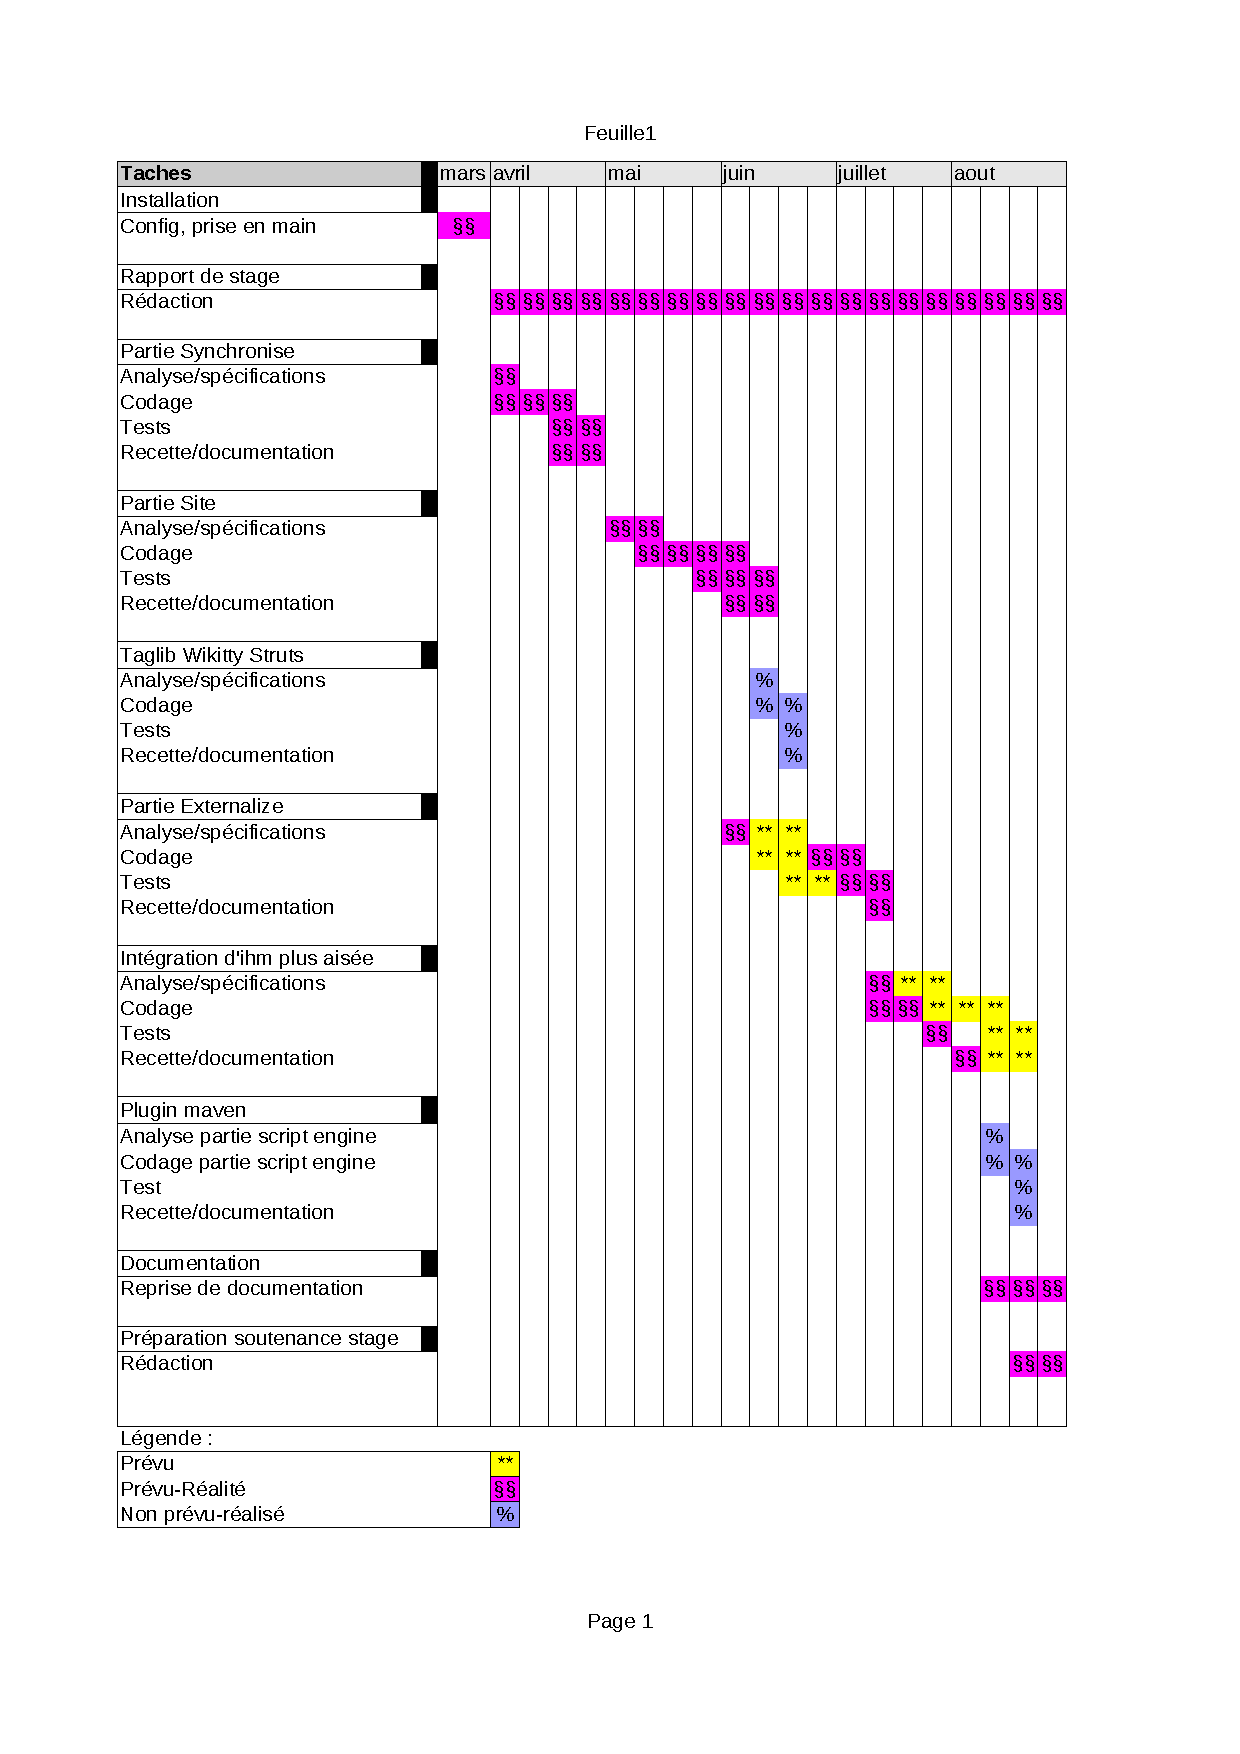
\includepdf{ressources/planningprev2.pdf} 


